% -*- TeX:de -*-
\NeedsTeXFormat{LaTeX2e}
\documentclass[12pt,a4paper]{article}
\usepackage[english]{babel} % german text
\usepackage[DIV12]{typearea} % size of printable area
\usepackage[T1]{fontenc} % font encoding
%\usepackage[latin1]{inputenc} % most likely on Windows
\usepackage[utf8]{inputenc} % probably on Linux
\usepackage{multicol}
% PLOTTING
\usepackage{pgfplots}
\usepackage{pgfplotstable}
\usepackage{url}
\usepackage{graphicx} % to include images
\usepackage{tikz}
\usepackage{subfigure} % for creating subfigures
\usepackage{amsmath} % a bunch of symbols
\usepackage{amssymb} % even more symbols
\usepackage{booktabs} % pretty tables
\usepackage{makecell} % multi row table heading
% a floating environment for circuits
\usepackage{float}
\usepackage{caption}
\usepackage{hyperref}

% Title Page command
\newcommand{\HRule}{\rule{\linewidth}{0.5mm}}

%\newfloat{circuit}{tbph}{circuits}
%\floatname{circuit}{Schaltplan}
% a floating environment for diagrams
%\newfloat{diagram}{tbph}{diagrams}
%\floatname{diagram}{Diagramm}
\pgfplotsset{compat=1.8}
\selectlanguage{english} % use german


\begin{document}
%%%%%%% DECKBLATT %%%%%%%
\begin{titlepage}
\begin{center}

% Upper part of the page. The '~' is needed because \\
% only works if a paragraph has started.

\includegraphics[scale=0.75]{./unilogo}~\\[2cm]

\textsc{\LARGE University of Vienna }\\[0.5cm]
\textsc{\LARGE Faculty of Physics}\\[1.5cm]
\textsc{\Large Quantum optics practical course}\\[0.5cm]

% Title
\HRule \\[0.4cm]
{ \huge \bfseries Radiaton Pressure}\\[0.4cm]

\HRule \\[1.5cm]

% Author and supervisor
\begin{minipage}{0.4\textwidth}
\begin{flushleft} \large
\emph{Author:}\\
Johannes \textsc{Kurz}\\
\emph{Group:}\\
\textsc{Braun, Donabaum, Kurz}\\
\end{flushleft}
\end{minipage}
\begin{minipage}{0.4\textwidth}
\begin{flushright} \large
\emph{Supervisor:} \\
Witlef \textsc{Wieczorek}
\end{flushright}
\end{minipage}

\vfill

% Bottom of the page
{\large 31.10.2014}

\end{center}
\end{titlepage}
%%%%%%% DECKBLATT ENDE %%%%%%%
\pagebreak
\setlength{\columnsep}{30pt}


\begin{abstract}
\noindent In this experiment, a helium-neon-laser is built and characterized. We describe the building process, from a set of available predefined components, as well as problems and their workarounds.\\
Furthermore polarization, shape of the beam and free spectral range are measured in order to calculate the characterizing parameters of the Gaussian beam.


\end{abstract}

\begin{multicols}{2}

%%%%%%%%%%%%%%%%%%%%%%%%%%%%%%%%%%%%%%%%%%%%%%%%
%\begin{figure}[H]
% \centering
% \includegraphics[scale=0.35]{./data/beugung.png}
% \caption{Beugungsmuster Einzelspalt (echtes Foto; schwarz durch weiß ersetzt)}
% \label{fig:beugungsmuster}
%\end{figure}



%\begin{figure}[H]
% \centering
% \pgfplotstabletypeset[
% columns={abstand, n},
% col sep=&,
% columns/abstand/.style={precision=2, zerofill, column name=\makecell{$Abstand$\\$(\pm 0.05)[mm]$} },
% columns/n/.style={column name=\makecell{$n$\\$(Ordnung)$}, precision=0},
% every head row/.style={before row=\hline,after row=\hline\hline},
% every last row/.style={after row=\hline},
% every first column/.style={column type/.add={|}{} },
% every last column/.style={column type/.add={}{|} }
% ]{
% abstand & n
% 12.9 & 1
% 24.45 & 2
% 37.40 & 3
% 49.35& 4
% 62.45 & 5
% 74.45 & 6
% 87.45 & 7
% 100.25 & 8
%
% }
% \caption{Messwerte Einzelspalt}
% \label{tab:werte_einzelspalt}
%\end{figure}

%%%%%%%%%%%%%%%%%%%%%%%%%%%%%%%%%%%%%%%%%%%%%%%%
%%%%%%%%%%%%%%%%%%%%%%%%%%%%%%%%%%%%%%%%%%%%%%%%

%\section{Helium-Neon-Laser}



%%%%%%%%%%%%%%%%%%%%%%%%%%%%%%%%%%%%%%%%%%%%%%%%
%%%%%%%%%%%%%%%%%%%%%%%%%%%%%%%%%%%%%%%%%%%%%%%%
\section{Theory}
 %\cite{physikwiki}.
A $laser$ is a light source, distinguished by its spatial and temporal coherence.\\
Spatial coherence means, the (usually very narrow) beam preserves it's profile over long distances (for example allowing for the precise dot produced by a laser pointer).\\
Temporal coherence shows in a very narrow frequency-spectrum of the beam (ideally monochromatic) and its polarization.\\

\subsection{Working principle}
\noindent Since a laser produces its output by "amplifying light through stimulated emission", it is built from some sort of \textbf{gain medium} (he-ne-mixture in this experiment) that is excited: This process is called \textbf{pumping} and is usually accomplished by another light-source or, as in this case, by an applied voltage.\\
The atoms of the he-ne-gas get excited to a higher energetic state. This state is not random, but highly correlated to the frequency of the e-field generated by the voltage, hence most of the excited atoms are in the same (or a few frequency-wise neighboring states). If an atom transitions back to its lower energy state, it emits a photon of the energy-difference. These photons can also be absorbed by other atoms and excite them. Since the probability of these transition is greatly increased by the pumping-process, this is called \textbf{stimulated emission}.
If the system is in a state of \textit{population inversion}, meaning that more atoms are in an excited state than are in ground state, more photons are emitted than absorbed and the light gets amplified.\\


\begin{figure}[H]
 \centering
 \includegraphics[scale=0.35]{./figures/HeNe_schematic.png}
 \caption{schematic drawing of a HeNe-laser $[3]$}
 \label{fig:hene-schematic}
\end{figure}

The gain medium is placed in an optical resonator (or 'cavity'), that consists of 2 mirrors, 1 that reflects (ideally) all photons back into the medium and another one with a (small) transmittance.\\
The photons bounce back and forth between the 2 mirrors and possibly excite the atoms again, thus producing a great amount of photons with same energy and impulse, leading to a coherent beam of photons leaving through the slightly transmissive mirror.\\

\noindent The pumping energy has to be large enough to overcome losses because of photons of other frequencies (that do not resonate) and material imperfections.\\

\subsection{Characterization and Measurements:}

\textbf{Polarization:}\\
The laser-beam should be highly linear polarized. Part of this experiment is to quantify the polarization by determining its visibility:
$$V = \frac{P_{max}-P_{min}}{P_{max}+P_{min}}$$
where $P_{max}$ and $P_{min}$ are the minimum (or maximum) intensities that pass through a polarizing beam-splitter (PBS) after a half-wave-plate is applied in different angles.\\

\noindent \textbf{Beam-Shape:}

\begin{figure}[H]
 \centering
 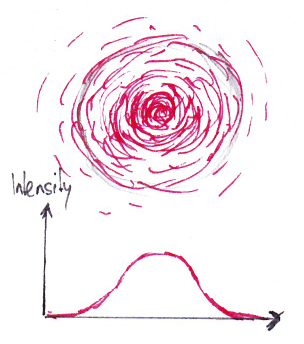
\includegraphics[scale=1.3]{./figures/gaussian_profile.png}
 \caption{Profile of a Gaussian Beam}
 \label{fig:gauss_profile}
\end{figure}


The beam emitted from the he-ne-laser is approximately a Gaussian-Beam. The intensity-distribution in the beam-profile follows a Gauss-distribution, and the beam-waist expands at a narrow angle.\\
The shape of the beam can thus be characterized by 2 parameters: the smallest beam-waist $\omega_0$ and the angle of its divergence. Furthermore we will try to verify a nearly circular profile by looking at the (gaussian) intensity distribution of the profile in 2 axis.\\

\begin{figure}[H]
 \centering
 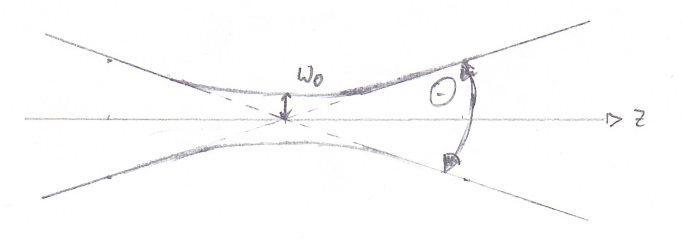
\includegraphics[scale=0.70]{./figures/gaussian_beam.png}
 \caption{Shape of a Gaussian Beam}
 \label{fig:gauss_beam}
\end{figure}

\noindent \textbf{Free spectral range - FSR}\\
The FSR is the difference in frequency between the modes of an optical cavity. There's resonance for waves of which the wavelength times an integer equals cavity length (these are called modes or standing waves).\\
So the FSR is a property of the cavity and dependent on its length.
$$\nu_{FSR} = \frac{c}{2L}$$
c... speed of light \\
L... cavity-length\\


\noindent The photons emitted from the atoms in the gas have certain preferred wavelengths, but not the sharp spectrum of the laser-beam. These wavelength cover about 3 to 4 modes of the cavity, resulting in a beam of (nearly) only those frequencies.\\
Since it is difficult in this experimental setup to measure the cavity-length precise enough, we will also apply 2 other methods, using the 3 wavelengths of the self-built laser:\\

\noindent One method makes use of a Fabry-Perot-Interferometer, a cavity similar to the laser's, where the position of one mirror is changeable by applying voltage to a piezo-crystal. By sweeping through different lengths of the reference cavity, one measures only then sharp intensity peaks, when its resonance matches an emitted mode of the laser.\\
Knowing the FSR of the reference cavity, one can determine the FSR of the laser-cavity. The velocity of the sweep has to be reasonable fast to not change the FSR of the measurement-cavity in the process.\\

\noindent A 3rd method is to measure the beat signal between 2 emitted wavelengths in a spectrum-analyzer. Since the frequencies themselves are to high and close together to measure their difference directly, one can make use of the much slower beat-signal produced by the superposition of different modes. The frequency of the beat-signal equals the frequency-difference of the 'beating signals' and therefore the FSR.

\noindent \textbf{Cavity Finesse:}
The cavity-finesse quantifies the quality of a cavity, it's the ratio between the FSR and the width of a single resonance-peak. Since it also matches the mean number of oscillations the photons do, before leaving the cavity, it can also be calculated from the reflectivity of the transmitting mirror (assuming the other one has a reflectivity of 1).
$$F = \frac{\pi \cdot R}{\sqrt{1 - R}} = \frac{\nu_{FSR}}{\Delta \nu}$$
F... Finesse\\
R...reflectivity\\
$\Delta \nu$ ... width of cavity resonance\\

\noindent \textbf{Stability-criterion of the cavity:}\\
In reality no alignment could be as perfect as to let the beam bounce between to parallel straight mirrors, so curved mirrors have to be used. This places a restriction on the cavity length:
$$0 \le g_1*g_2 \le 1$$
$$g_{1,2} = 1 - \frac{d}{R_{1,2}}$$
where\\
d ... cavity-length\\
$R_{1,2}$ ... radius of curvature of the mirrors\\

%%%%%%%%%%%%%%%%%%%%%%%%%%%%%%%%%%%%%%%%%%%%%%%%
%%%%%%%%%%%%%%%%%%%%%%%%%%%%%%%%%%%%%%%%%%%%%%%%
\section{Experimental Setup}
\subsection{Building the Laser}
The whole setup is built on an optical table (breadboard) and matching optical elements (mostly by Thorlabs).\\
The laser itself consists of a gas-tube (filled with an helium-neon-mixture) with electrical contacts on both ends to apply high-voltage, and a slightly transmissive mirror on an adjustable mirror-mount. The fully reflective mirror is already built-in the tube.
For the construction of the laser we used an additional laser (alignment-laser) and 2 mirrors on adjustable mounts to couple into the cavity.\\
One of the 2 mirrors is placed quite far away from the gas-tube, so that changes of its angle result in translational shifts of the laser-point on the cavity-mirror. The second one is placed fairly near the cavity to produce mainly an angular shift, thus dividing the 4 degrees of freedom (2 angular, 2 translational).\\
It's recommended to adjust the alignment-laser so that the beam gets reflected back into the laser in addition to passing through the whole tube. The longer beam-path back gives a finer measurement of the correct angle, than just the pass-through-requirement.\\

\begin{figure}[H]
 \centering
 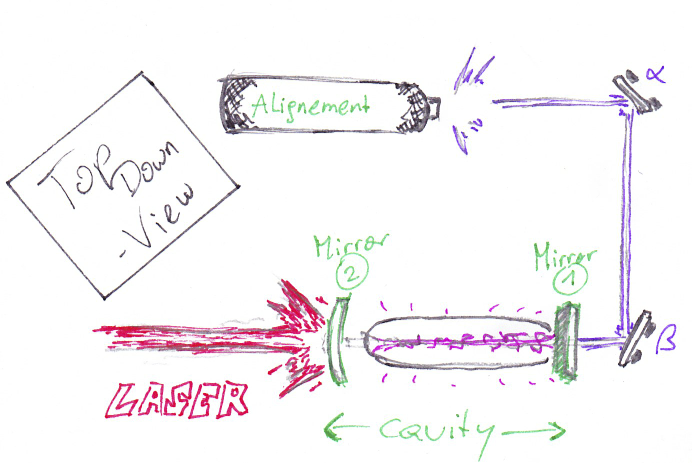
\includegraphics[scale=0.65]{./figures/exp_setup.png}
 \caption{Experimental Setup}
 \label{fig:exp_setup}
\end{figure}

\noindent After the pre-alignment, the second cavity-mirror is placed at the cavity-output. The distance to the other mirror has to fulfill the stability-requirement of the cavity and should be es orthogonal as possible to the beam-path.\\
After applying voltage from a power-supply via the 2 contacts on the tube, the gas should start to glow and the laser possibly already works. Usually this is not the case, but one should 'search' for the right angle of the curved mirror.\\
If there's no laser-beam after tilting the mirror, then the pre-alignment has to be checked, improved or done again. Also different cavity-lengths can be tried:\\
The shorter, the safer, but there's a possibility of arc discharge, if the mirror-mount is too close to the contacts.

\subsection{Measurements}
\textbf{Polarization:}\\
The Polarization is measured by placing first a rotatable half-wave-plate ($\lambda$/2-plate) and behind a polarizing beam-splitter into the beam-path. A power-meter is used to measure the intensity behind the PBS, either transmitted or reflected. The $\lambda$/2-plate changes the direction of the polarization and for different rotations (here every 10$^\circ$) the intensity after the PBS is measured. The resulting curve should oscillate between 2 intensities and after a sine-fit $P_{max}$ and $P_{min}$ can be used to calculate the visibility of the Polarization.\\

\noindent \textbf{FSR:}\\
For the free-spectral-range-measurement by cavity length, a simple ruler is used to measure the length, thus being very imprecise (the exact position of the mirror-surfaces is hidden in the mounts).\\
To couple into the Fabry-Perot-interferometer as well as into the optical fiber leading to the diode (for spectroscopy) a setup of 2 mirrors for translation and beam-angle is used, similar to that in the pre-alignment.\\

\begin{figure}[H]
 \centering
 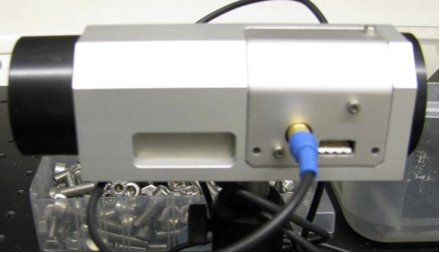
\includegraphics[scale=0.9]{./figures/FPI.png}
 \caption{Fabry-Perot-Interferometer, image from [1]}
 \label{fig:FPI}
\end{figure}

\noindent The piezo-crystal inside the FPI is controlled by a high-voltage-amplifier, of which the output is modulated by a trigger-signal from an oscilloscope. That way one can plot the intensity measured against the frequencies of the peaks.\\
The spectroscopy is done with a photo-diode (custom-made-circuit was provided) and an A/D-converter.\\

\noindent The cavity-finesse can be calculated either using the FSR and width of the resonance-peaks or 
the reflectivity of the output mirror.\\
To measure the reflectivity the mirror is simply put in front of the alignment-laser with a power-meter behind it. additional the power of the laser without mirror has to be measured. The ratio between the 2 gives the reflectivity.\\
It is good, to wait for a while, so the power of the laser stabilizes, and to tilt the mirror slightly as to not create a resonator between laser and mirror.\\

\noindent \textbf{Beam-shape and profile}
Both, the profile and the shape of the beam are measured by using the same apparatus:\\
A slit in a plate, mounted on a translation-stage equipped with a micrometer-screw(Fig. \ref{fig:shape_measure})

\begin{figure}[H]
 \centering
 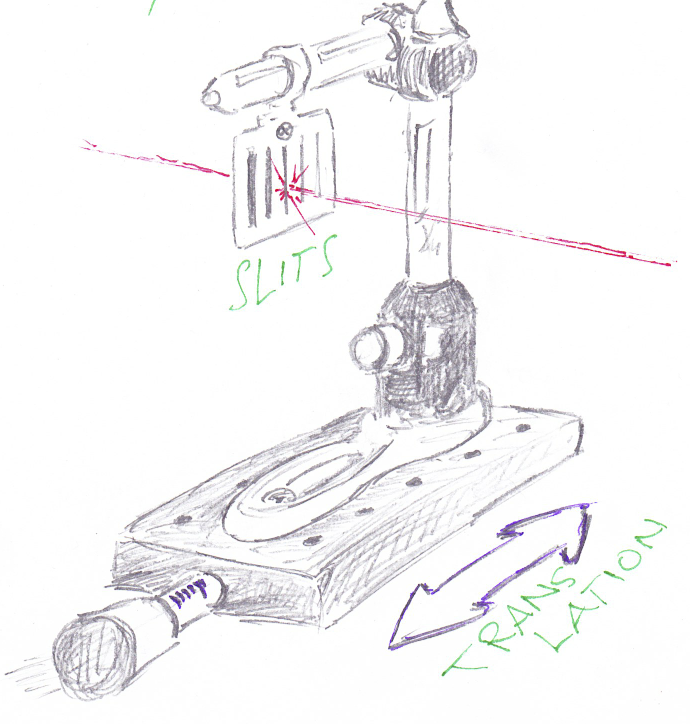
\includegraphics[scale=0.7]{./figures/shape_measure.png}
 \caption{Slit mounted on a translation-stage}
 \label{fig:shape_measure}
\end{figure}

The measurement is taken by sweeping the slit through the beam and taking intensity-measurements of the passing light at discrete positions. A Gaussian-function is fitted through the data points.\\
This is done in horizontal and vertical direction at one distance to the laser, to check if the beam is circular or elliptical.\\
Then this process is taken at several distances from the laser (only horizontal, the profile-shape doesn't change). By comparing the FWHM of the Gauss-fits at different distances, the shape of the beam is measured.\\
The smaller the slit, the better the resolution, but it is necessary to check, if the slit is so small that a diffraction pattern occurs.
%%%%%%%%%%%%%%%%%%%%%%%%%%%%%%%%%%%%%%%%%%%%%%%%
%%%%%%%%%%%%%%%%%%%%%%%%%%%%%%%%%%%%%%%%%%%%%%%%

\pagebreak
\section{Results}


\subsection{Reflectivity of the output mirror}
\textbf{1st measurement:}\\
no mirror: $I_{1,without} = (19.50 \pm 0.01)mW$\\
mirror: $I_{1,with} = (0.26 \pm 0.01)mW$\\
reflectivity: $R_1 = 1-(I_{1,with}/I_{1,without})$\\
$R_1 = (0.987 \pm 0.001)$\\

\noindent \textbf{2nd measurement:}\\
no mirror: $I_{2,without} = (20.31 \pm 0.01)mW$\\
mirror: $I_{2,with} = (0.27 \pm 0.01)mW$\\
reflectivity $R_2 = (0.987 \pm 0.001)$\\
$$R = (0.987 \pm 0.001)$$

%uncertainty times 2 because of other influences


\subsection{Polarization}
\begin{figure}[H]
 \centering
 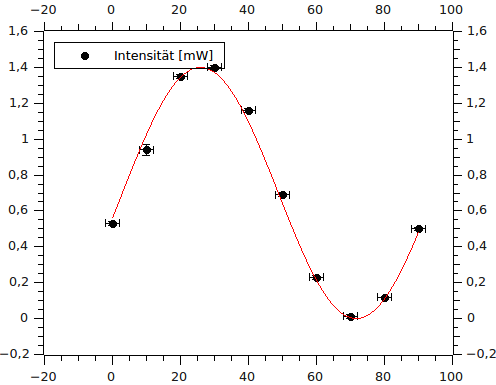
\includegraphics[scale=0.46]{./figures/pol_sinfit.png}
 \caption{Polarization measurement\\ \textbf{x-axis:}Rotation of $\lambda/2$-plate (deg)\\
\textbf{y-axis:}Intensity(mW)}
 \label{fig:shape_measure}
\end{figure}

\noindent total laser-intensity (without $\lambda$/2 and PBS): $I = (1.50\pm 0.02)mW$\\
$P_{max} = (1.400 \pm 0.005)mW$\\
$P_{min} = (0.012 \pm 0.005)mW$\\
$$Vis = (0.9858 \pm 0.0070)$$

% uncertainty round up


\subsection{Beam-shape and profile}

\begin{figure}[H]
 \centering
 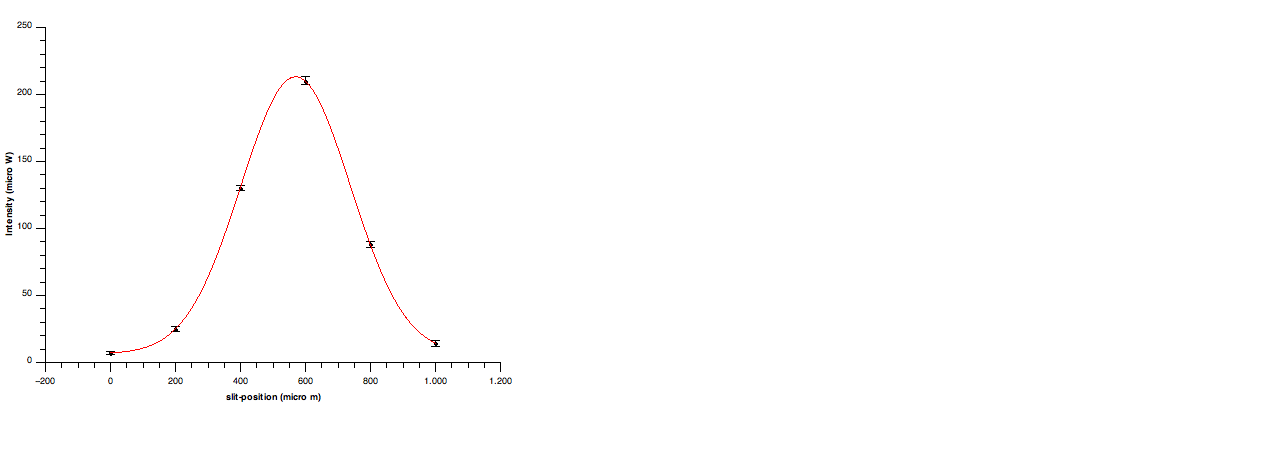
\includegraphics[scale=0.46]{./figures/beamprofile_horiz_43cm.png}
 \caption{slitscan-measurement, horizontal, distance: 43cm from the fixed mirror}
 \label{fig:shape_measure}
\end{figure}

\begin{figure}[H]
 \centering
 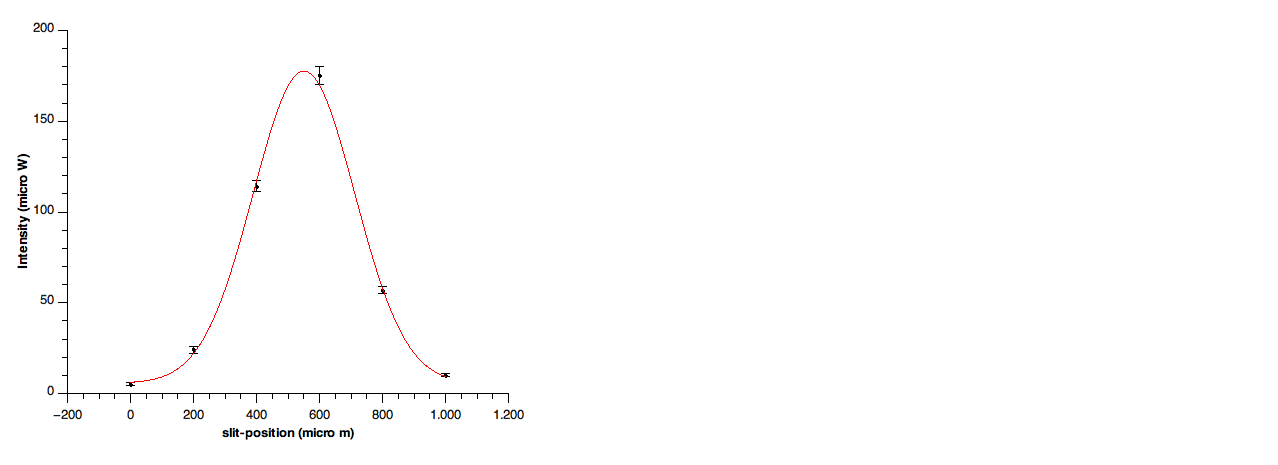
\includegraphics[scale=0.46]{./figures/beamprofile_vertic_43cm.png}
 \caption{slitscan-measurement, vertical, distance: 43cm from the fixed mirror}
 \label{fig:shape_measure}
\end{figure}


\noindent \textbf{beam-profile:}\\
diameter of the beam taken from FWHM of the gauss-fit:\\
\O$_{hor} = (336,76 \pm 0.79) \mu m$\\
\O$_{vert} = (323 \pm 11) \mu m$
$$Ratio_{vert/hor}=(0.959 \pm 0.033)$$
The beam has a nearly circular profile.\\

\noindent \textbf{beam-shape:}\\
Similar measurements and fits at  few positions:\\
\O$_{29cm} = (336,76 \pm 0.79) \mu m$\\

\begin{figure}[H]
 \centering
 \pgfplotstabletypeset[
 columns={distance, diameter},
 col sep=&,
 columns/distance/.style={precision=0, zerofill, column name=\makecell{$distance$\\$\pm 5(mm)$} },
 columns/diameter/.style={column name=\makecell{$diameter$\\$(\mu m)$}, string type},
 every head row/.style={before row=\hline,after row=\hline\hline},
 every last row/.style={after row=\hline},
 every first column/.style={column type/.add={|}{} },
 every last column/.style={column type/.add={}{|} }
 ]{
distance & diameter
 290 & $324.4 \pm 5.7$
 305 & $335.3 \pm 2.0$
 430 & $336.76 \pm 0.79$
505 & $359.8 \pm 5.2$
605 & $412.8 \pm 9.5$
705 & $443.9 \pm 9.6$


 }
 \caption{beamdiameter at various distances}
 \label{tab:diameter_table}
\end{figure}


\begin{figure}[H]
 \centering
 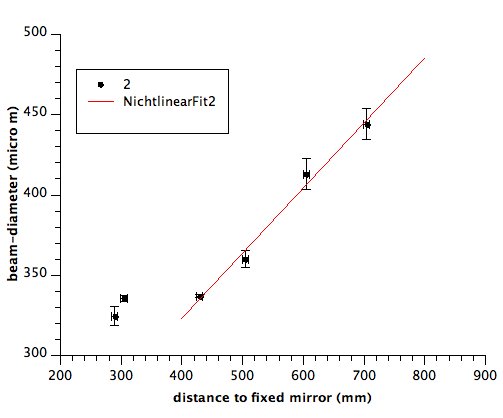
\includegraphics[scale=0.46]{./figures/beamshape_linfit.png}
 \caption{beam-diameter vs measurement-position}
 \label{fig:beamshape_linfit}
\end{figure}

\noindent $slope = (0.405 \pm 0.033) \times 10^{-6}$
$$\Theta_{div} = (23.2 \pm 0.19)^{\circ} \times 10^{-6}$$

\subsection{Free spectral range}
\textbf{FSR by cavity length:}\\
$L = (0.23 \pm 0.01)m$
$$\nu_{length} = \frac{c}{2\cdot L}=(0.652\pm 0.029)GHz$$

\noindent \textbf{FSR by Fabry-Perot-Interferometer:}\\

\begin{figure}[H]
 \centering
 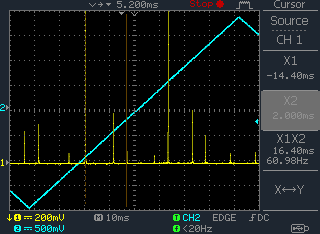
\includegraphics[scale=0.90]{./figures/FPI_osci.png}
 \caption{oscilloscope-measurement from an FPI}
 \label{fig:FPI_osci}
\end{figure}

\begin{figure}[H]
 \centering
 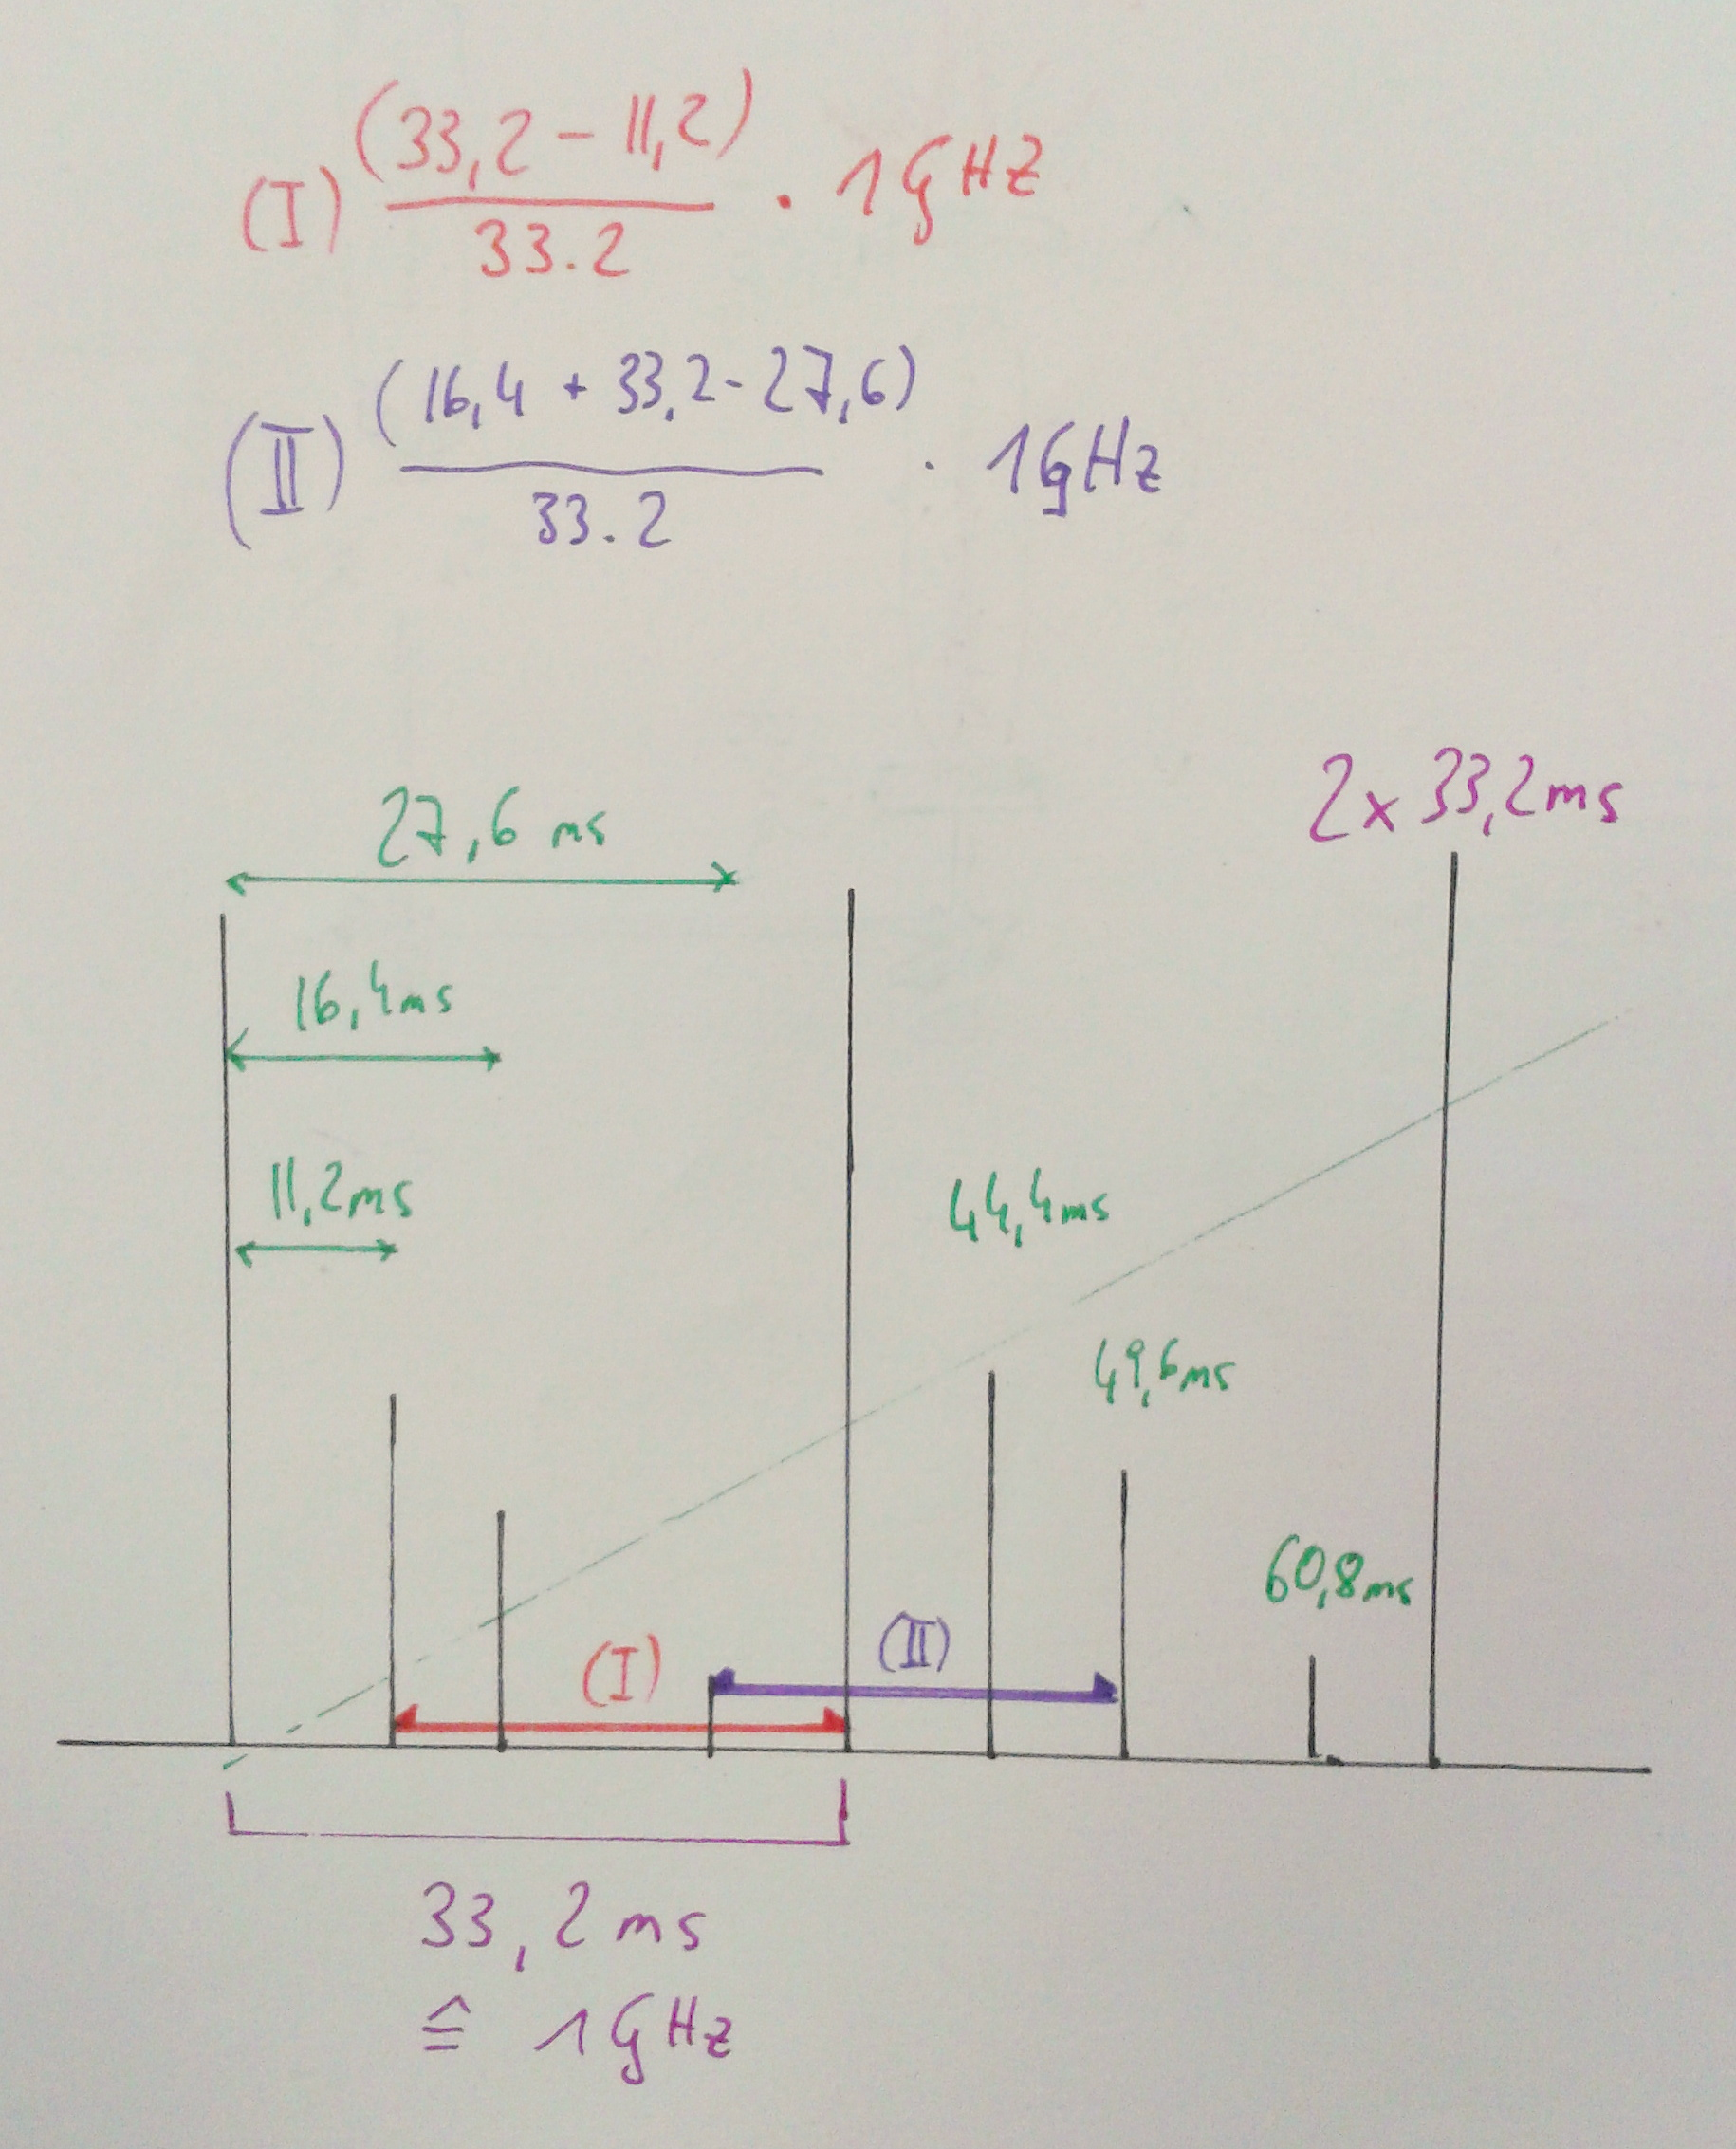
\includegraphics[scale=0.11]{./figures/FPI_explain.jpeg}
 \caption{evaluation of oscilloscope-data}
 \label{fig:FPI_explain}
\end{figure}

\noindent Since in reality adjacent modes are not necessarily beside each other on the oscilloscope-measurement (dependent on the 1GHz FPI-FSR), the evaluation can be tricky. Using the FSR-estimate from length measurement to find the right modes first, one can later proof the validity by finding more than one mode-combination, that give the same FSR (Fig. \ref{fig:FPI_explain}).\\
\\
Positions on the time scale (from left to right:)\\
$Peak_1=(0 \pm 0.1)ms$\\
$Peak_2=(11.2 \pm 0.1)ms$\\
$Peak_3=(16.4 \pm 0.1)ms$\\
$Peak_4=(27.6 \pm 0.1)ms$\\
\\
$FSR_1 = (0.6627 \pm 0.0032)GHz$\\
$FSR_2 = (0.6627 \pm 0.0053)GHz$

$$\nu_{FPI} = (0.6627 \pm 0.0062)GHz$$

\noindent \textbf{FSR by beat-signal}\\

\begin{figure}[H]
 \centering
 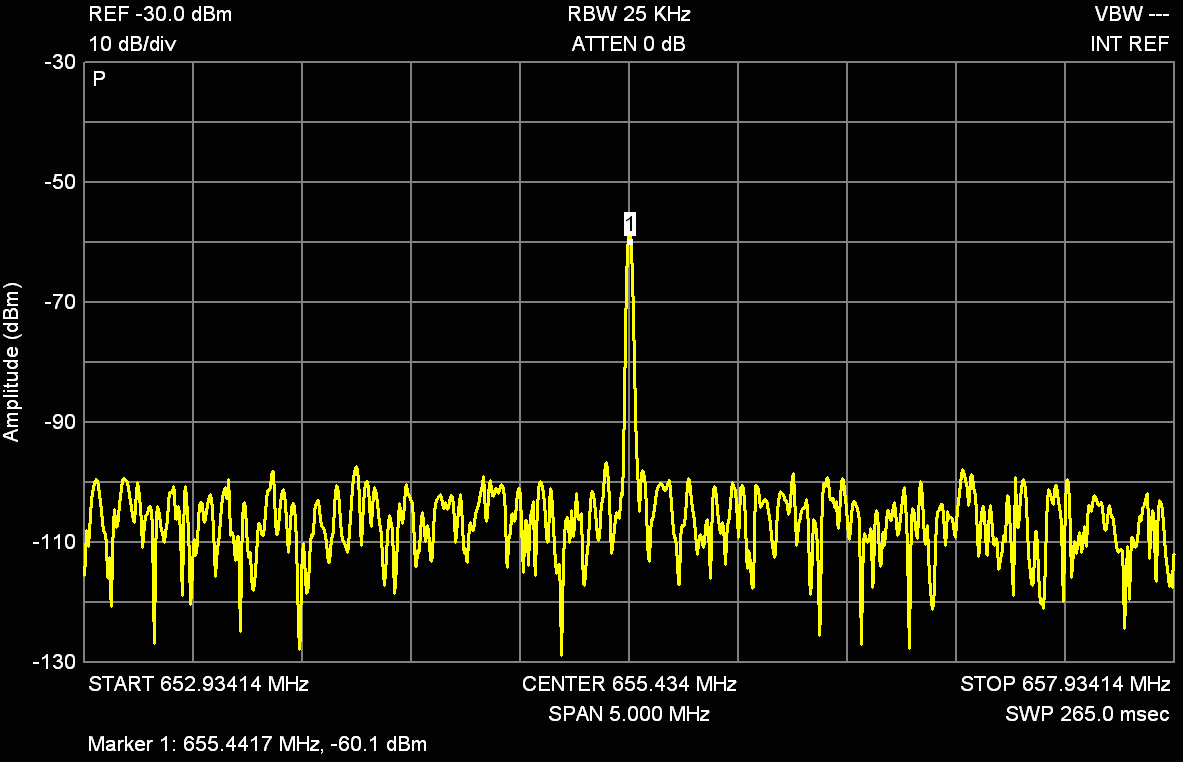
\includegraphics[scale=0.18]{./figures/655mhz_peak1.png}
 \caption{measurement of the beat-signal between the laser-modes}
 \label{fig:beatsignal}
\end{figure}

$\nu_{beat}=|f_1 - f_2|= FSR$
$$\nu_{beat}=(0.655 \pm 0.002)GHz$$


\subsection{Cavity Finesse}
$R = (0.987 \pm 0.001)$
$$F = (240 \pm 19)$$ 
$\approx$ 2.58 $\%$ roundtrip-loss\\
\\
\textit{(All raw-data is stored in [2])}

%\cite{github}


%%%%%%%%%%%%%%%%%%%%%%%%%%%%%%%%%%%%%%%%%%%%%%%%
%%%%%%%%%%%%%%%%%%%%%%%%%%%%%%%%%%%%%%%%%%%%%%%%

\section{Discussion}
\subsection{Laser Setup}
We built the laser for about 6 times for various reasons (losing the cavity while optimizing, changes over night, deliberately starting from scratch to get it better, etc.). It is notable that there are great differences in output-intensity just from slight variations. To get consistent measurements, it is probably better to practice and build the laser multiple times and try to get a stable functioning laser with as minimal faults as possible, before doing the measurements.\\
Furthermore some influences, like temperature shifts and changing currents are not easily controllable under the time- and equipment-constraints during the course. So improving the mounts, swapping posts and post-holders for better ones, if available, and working precise, becomes important.\\
Since this course was our first introduction to really working with optical elements, we could certainly improve on this part.\\
\\
\subsection{Measurements}
\textbf{Reflectivity:}\\
Even though the setup for the reflectivity measurement of the output-mirror is fairly simple, there are quite some possibilities for faults and uncertainties:\\
The power of the alignment-laser is not stable enough, even after some warming-up. The slight tilt of the mirror, to avoid reflecting the beam back and forth and multiplying, proves to influence the data quite a bit, leading to the conclusion, that a greater uncertainty (than the resolution of the powermeter) has to be assumed: We use an uncertainty of $\pm 0.01$mW instead of 0.001mW (plus some fluctuations).\\
\\
\textbf{Polarization:}\\
The sinusoid fits the data well and leads to an expected result of nearly 100$\%$ linear Polarization. The  measurement could possibly be even improved by rotating the $\lambda$/2-plate the whole 360$^{\circ}$. We just checked, if the extremal-points repeat after every 90$^{\circ}$. Since the laser is not that stable and the fit is very precise, the uncertainties of the whole setup are assumed to be much greater than a mean value over 4 periods could compensate.\\
\\
\textbf{Beamshape}\\
The profile of the beam follows a gaussian distribution both in the horizontal as well as the vertical direction. Their ratio is nearly 1 meaning the shape of the beam-profile is nearly circular.\\
The uncertainty in the vertical direction is very large compared to the horizontal uncertainty.\\This stems for one from the vertical being the greatest uncertainty of all of these beam measurements (but only by a margin) as well as the horizontal measurement at that distance being especially precise (the uncertainty of the gaussian fit is much smaller than the others).\\
The great difference in uncertainty for comparing horizontal and vertical direction comes therefore from 'being lucky' with the horizontal measurement.\\
\\
The shape of the beam follows that of a gaussian-beam, as drawn in \ref{fig:gauss_beam}. Therefore the linear fit for determining the divergence angle $\Theta_{div}$ is only drawn over the second party of the data. At close range to the laser the beam does not diverge at the full angle.\\
\\
The measurement by slit and translation stage seems to be surprisingly precise and sturdy against influences from changing the distance (and thus shaking the whole setup while unscrewing the stage) and the imprecise distance measurement. The Gaussian fits seem to cancel out most of these disturbances.\\
\\
\textbf{FSR:}
All 3 measurements of the FSR are reasonable close inside their uncertainties. Beat-signal-result and the FPI-result barely touch though. The uncertainty of the beat signal was assumed greater than the resolution of the spectroscopy-software, since the spectrum fluctuated quite a bit (It is a beat signal of more than 2 frequencies).\\
Since the results are close together, we assume, that $\nu_{length}$ and $\nu_{beat}$ being very close together while $\nu_{FPI}$ just touching the same area, is a coincidence and cannot just lead to the conclusion of a fault in the FPI-measurement.\\
One would have to repeat the experiment and take extra care to try and see, if both are still that close together, while $\nu_{FPI}$ somewhat drifting away.


%%%%%%%%%%%%%%%%%%%%%%%%%%%%%%%%%%%%%%%%%%%%%%%%
%%%%%%%%%%%%%%%%%%%%%%%%%%%%%%%%%%%%%%%%%%%%%%%%
%\bibliography{protocol.bib}
%\bibliographystyle{plain}
\section{Bibliography}
$[1]$ Anleitung\\
$[2]$ data stored in \url{https://github.com/blackandcold/PR_Quantumoptics_Summer2014/tree/master/HeNeLaser}\\
$[3]$ %FSR-Illustration \url{http://en.wikipedia.org/wiki/Free_spectral_range}\\
HeNe-schematic, \url{http://en.wikipedia.org/wiki/Helium\%E2\%80\%93neon_laser}\\
DrBob, under GNU free documentation license


\end{multicols}
\end{document}